% !TEX root = ../main.tex
% Chapter 6

\chapter{Real-world results}

\label{Chapter6} % For referencing the chapter elsewhere, use~\ref{Chapter6}

\lhead{Chapter 6. \emph{Real-world results}} % This is for the header on each page - perhaps a shortened title

In this chapter we discuss the real-world data sets used for this research and the performance of our proposed algorithm on these data sets.
In \Cref{sec:data_sets} we discuss available data sets and argue that these are inappropriate for our research.
It is followed by an overview of the setup we have created to record our own continuous data sets in an unknown environment, both for in- and outdoor activities.
The series of activities performed are discussed in \Cref{sec:data_gathering}.
In that section we show typical plots of the inertial sensor data and stills from the video recordings.
That will illustrate the setting in which the activities are performed and the characteristics of continuous data.
Finally, the results of the algorithm are discussed in \Cref{sec:real_world_results}.
We will use the objective measures, introduced in \Cref{sec:artificial_data_quality_metrics}, and also give subjective claims on the performance of the algorithm applied to the real-world data.
Since the data sets used are real-world recordings, we will put emphasis on the latter type of quality measures \ie the subjective claims.

% !TEX root = ../../main.tex
\section{Data Sets}\label{sec:data_sets}
In the previous chapter we have applied our method to the artificial data sets from Camci~\cite{camci2010change} and Takeuchi and Yamanishi~\cite{takeuchi2006unifying}.
In this chapter we apply the method to real-world data sets.
The data sets come from inertial sensor data recorded during human activities, such as walking, running, ascending and descending stairs, and standing still.
To compare our results with other research, we have tried to apply our method to two commonly used data sets.
The first is the data from the \gls{wisdm} lab \cite{kwapisz2011activity}.
As an excerpt from the data in \Cref{fig:wisdm_excerpt} shows, the activities are recorded non-continuous.
Whilst this data set is convenient for activity classification, it does not allow for detection of change points.
Even if the gap between the activities would be removed, the transition segments between activities would still be missing and thus the data set would not reflect continuous recordings.
The other commonly used data set is the \gls{uci-har} from the Machine Learning Repository and originates from \cite{anguita2012human}.
As shown in an except in \Cref{fig:uci_annotated}, the labeling to the data segments seems to be incorrect.
Furthermore, it is not clear how the data is recorded and whether all activities are performed continuously.

\begin{figure}
\centering
  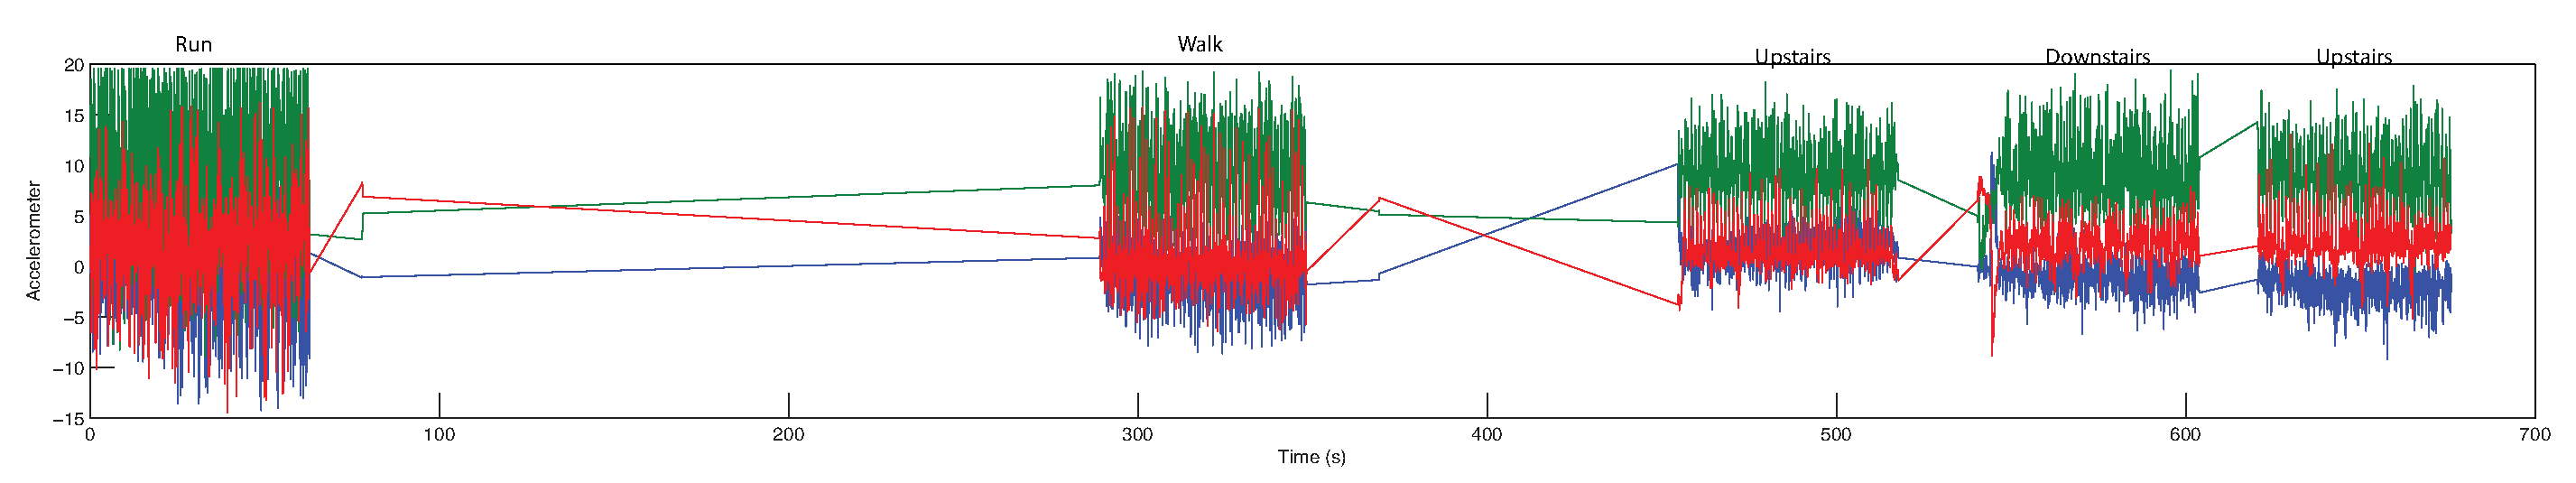
\includegraphics[width=1\textwidth]{./Figures/Chapter6/data_collection/wisdm_excerpt.eps}
  \caption[WISDM Excerpt]{Excerpt from the WISDM data set \cite{kwapisz2011activity}. First five activities for subject $33$ are displayed. Due to the discontinuous nature of the recordings, this data set can not be used for change detection.}
  \label{fig:wisdm_excerpt}
\end{figure}

\begin{figure}
\centering
  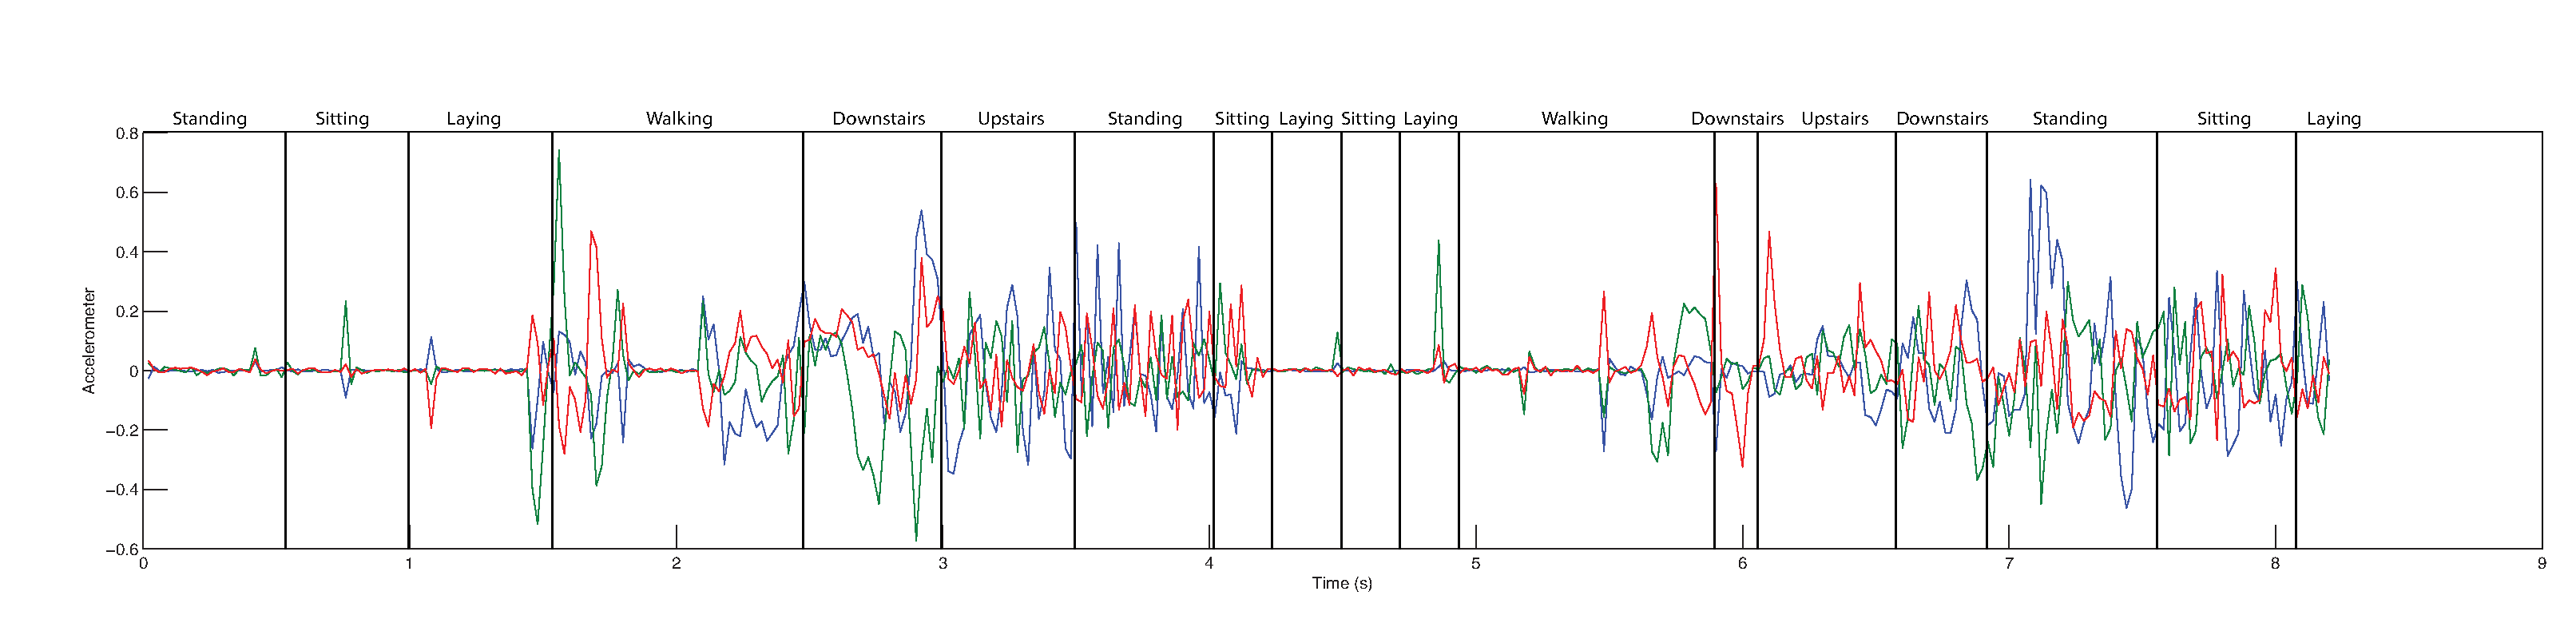
\includegraphics[width=1\textwidth]{./Figures/Chapter6/data_collection/uci_annotated.eps}
  \caption[UCI HAR Excerpt]{Excerpt from the UCI HAR data set \cite{anguita2012human}. The recorded training activities for subject $25$ are displayed. Due to the imprecise (and possibly incorrect) labeling and the short duration of activities, the data set can not be used for the change detection method as described in this thesis.}
  \label{fig:uci_annotated}
\end{figure}

Because of the above described shortcomings of commonly used data sets, we have decided to record activities by ourselves.
The following characterizing requirements were set for our data sets:
\begin{enumerate}
  \item The activities need to be performed and recorded in a continuous manner,
  \item The environment should be natural and uncontrolled, both in- and outdoor,
  \item The data should be clearly annotated, as objective as possible,
  \item The required hardware (and software) should be widely available.
\end{enumerate}

With these requirements in mind, we have created the following setup.
All activities were recorded by a smartphone worn on body in the right front pants pocket of the subject.
The used phones are the \textsc{HTC Sensation XE} and \textsc{HTC Desire}, running the \textsc{Android} smartphone operating system.
During the activities the inertial sensor data is recorded using a free application, \textsc{Sensor Logger}~\cite{sensorlogger}.
This application records the sensor data to \textsc{CSV} files, which are then transformed to \textsc{MATLAB} compatible files.
The constructed algorithm processes the data in an online manner (using only current and historic data).
The \textsc{MATLAB} implementation uses the \gls{svdd} library \textsc{dd\_tools} by Tax \cite{Ddtools2013}.
During the activities, the subject is recorded with a video camera to enable manual labeling and determination of the change points.
As illustrated in the top row of \Cref{fig:stills_subject_1_and_2}, the manual labeling is an ambiguous task.
In \Cref{fig:stills_subject_2_change_point} a transition between walking and running is shown.
It is impossible to determine the exact location of the change point and thus objective quality measures (such as the delay) are of less importance.

Using the video recordings, the data sets are manually annotated, as shown in the plots of \Cref{fig:plots_subject_1,fig:plots_subject_2,fig:plots_subject_3}.
The graphs display each from a single recording the inertial sensor values (see \Cref{tab:recorded_metrics} for explanation of the metrics), with manually annotated activities above the data.
The manually determined change points are used to draw quality conclusion over the algorithm's performance, by comparing it to the discovered change points.
All of the used data sets, including the video material and manual labeling, are made available to the public as \gls{almende-data} \cite{vlasveld2014acras} for further research.
The following section discusses the performed activities during the recordings.

% !TEX root = ../../main.tex
\section{Data Gathering}\label{sec:data_gathering}

\TODO{Use common data sets. The WISDM dataset is not usefull because it has no transitions, only very clear blocks of the same activities. Include a plot to illustrate the problem?}


\begin{figure}\label{fig:wisdm_excerpt}
\centering
  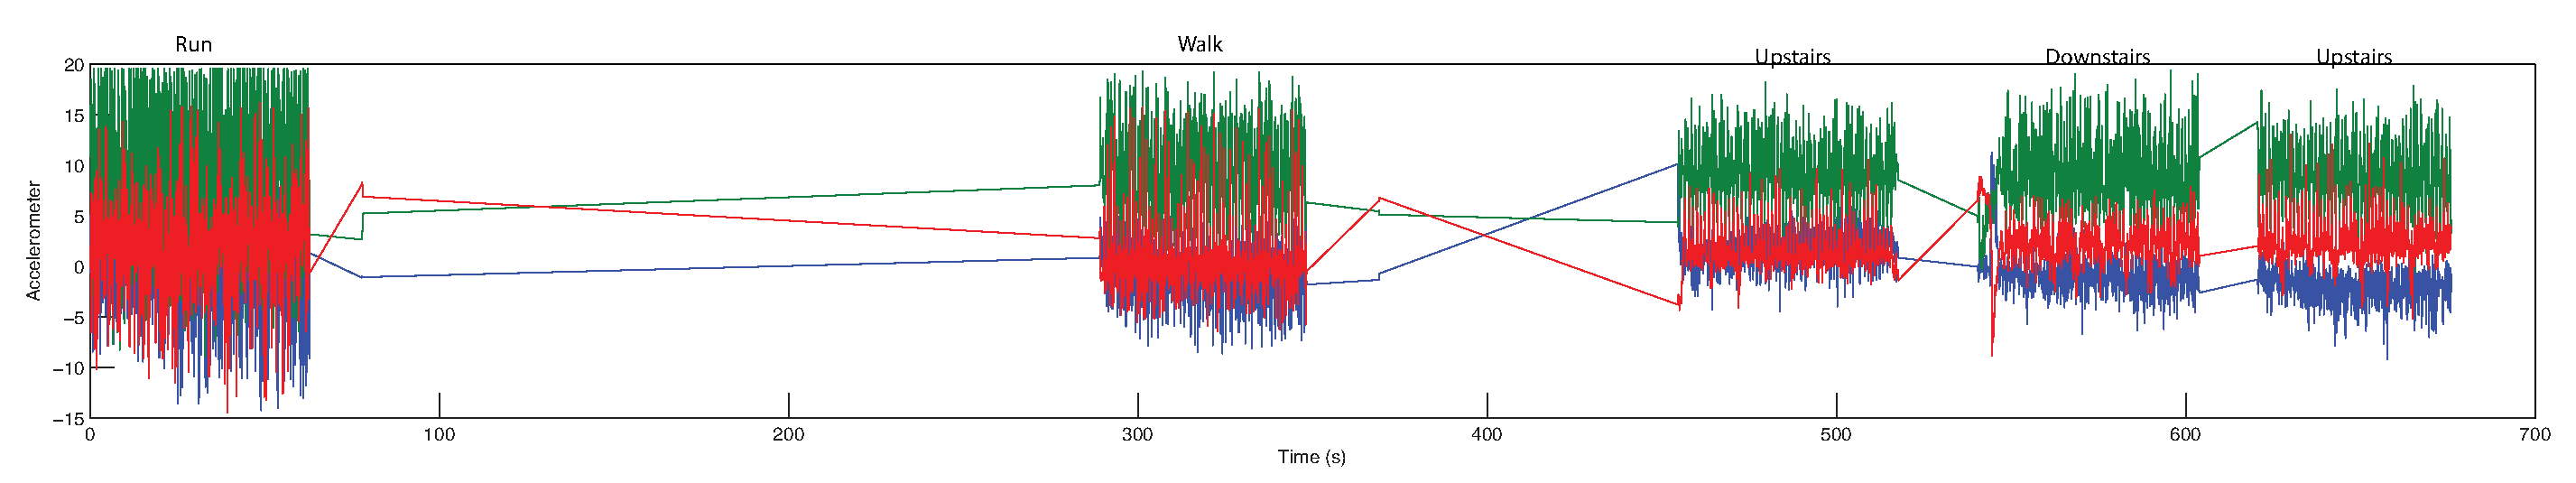
\includegraphics[width=1\textwidth]{./Figures/Chapter6/data_collection/wisdm_excerpt.eps}
  \caption[Jumping variance ratios]{Excerpt from the WISDM data set \cite{kwapisz2011activity}. First five activities for subject $33$ are displayed. Due to the discontinuous nature of the recordings, this data set can not be used for change detection.}
\end{figure}

%---- Run 1: walk-run-roemer
\begin{figure}
\centering
  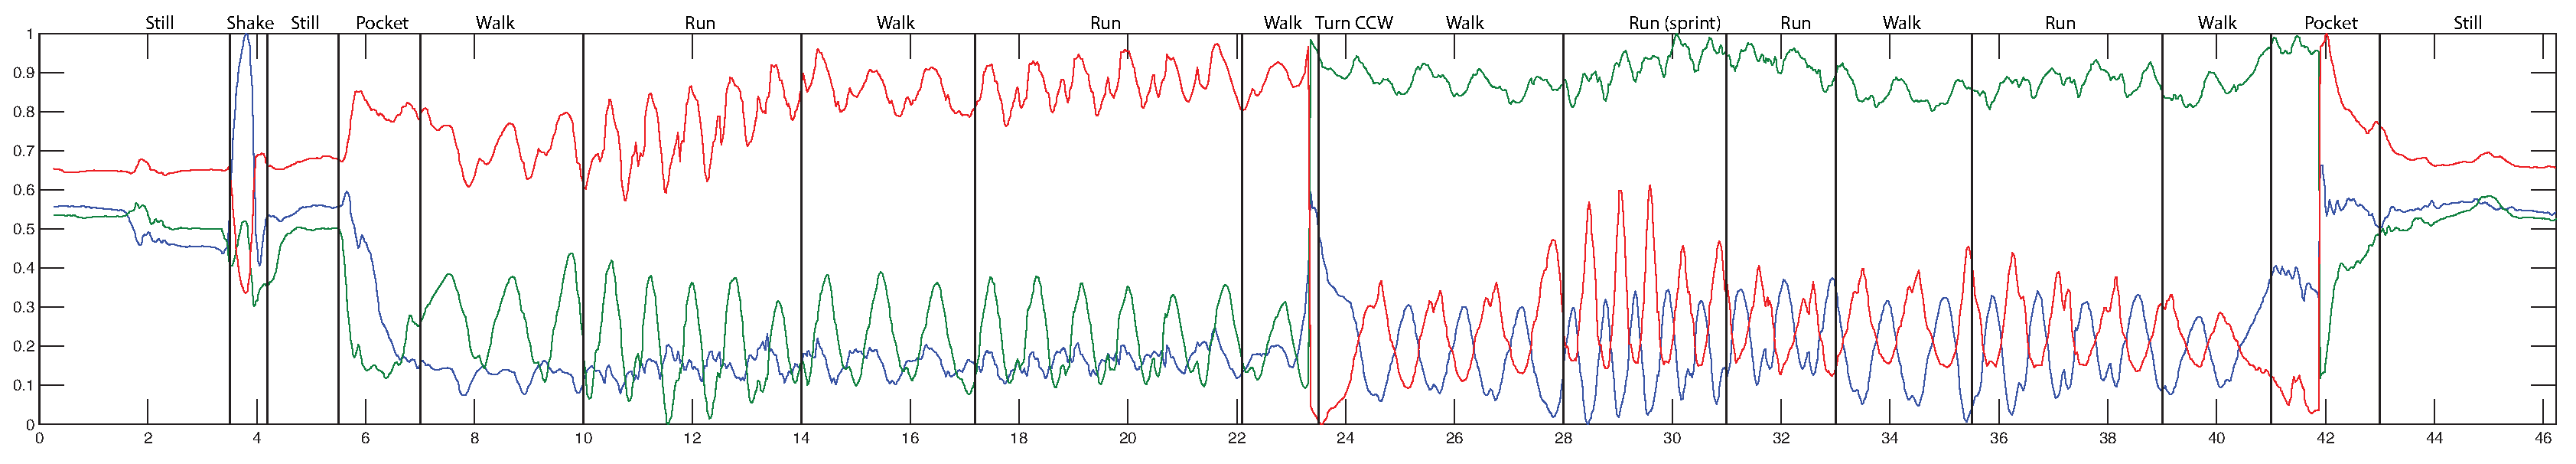
\includegraphics[width=1\textwidth]{./Figures/chapter6/data_collection/run-1-walk-run-roemer/data_plot_rot_annotated.eps}
  \caption[R1: rotation]{Run 1: Walk-run-roemer, rotation}
\end{figure}

\begin{figure}
\centering
  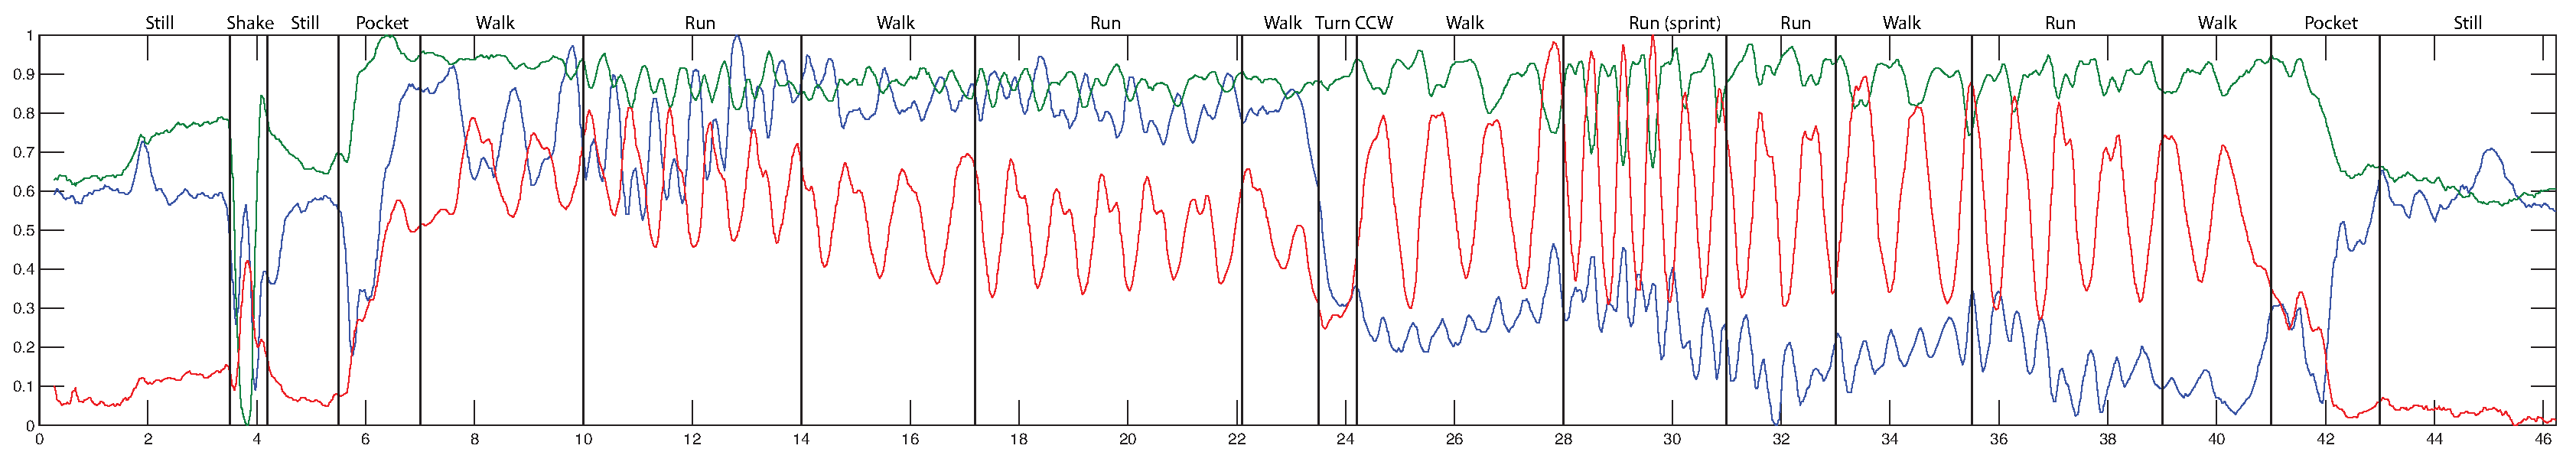
\includegraphics[width=1\textwidth]{./Figures/chapter6/data_collection/run-1-walk-run-roemer/data_plot_mag_annotated.eps}
  \caption[R1: mag]{Run 1: Walk-run-roemer, Mag}
\end{figure}

\begin{figure}
\centering
  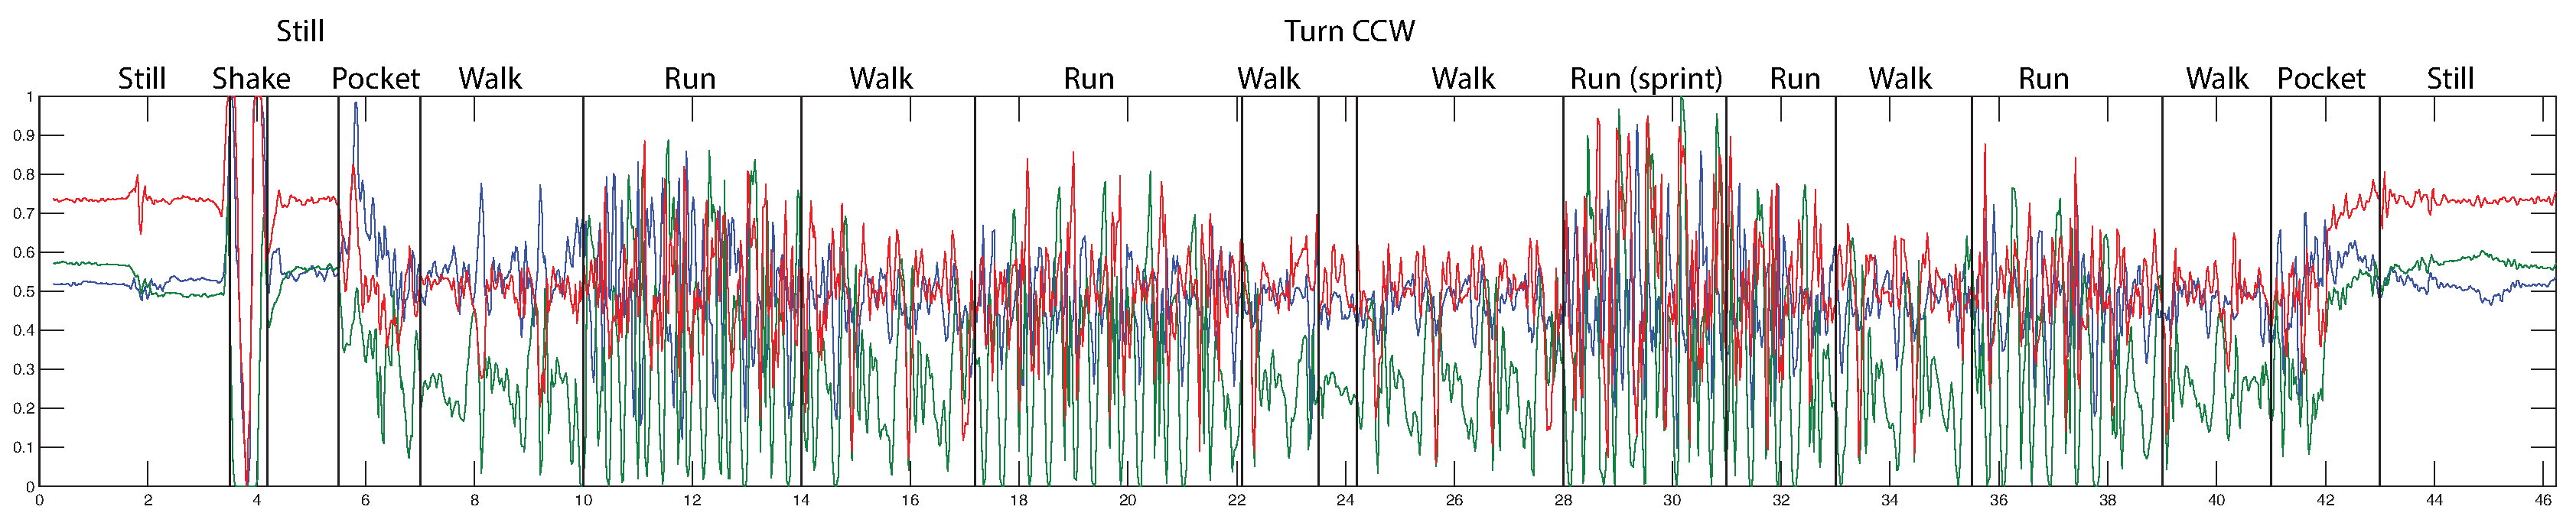
\includegraphics[width=1\textwidth]{./Figures/chapter6/data_collection/run-1-walk-run-roemer/data_plot_acc_annotated.eps}
  \caption[R1: accelerometer]{Run 1: Walk-run-roemer, accelerometer}
\end{figure}

%---- Run 2: walk-run-jos
\begin{figure}
\centering
  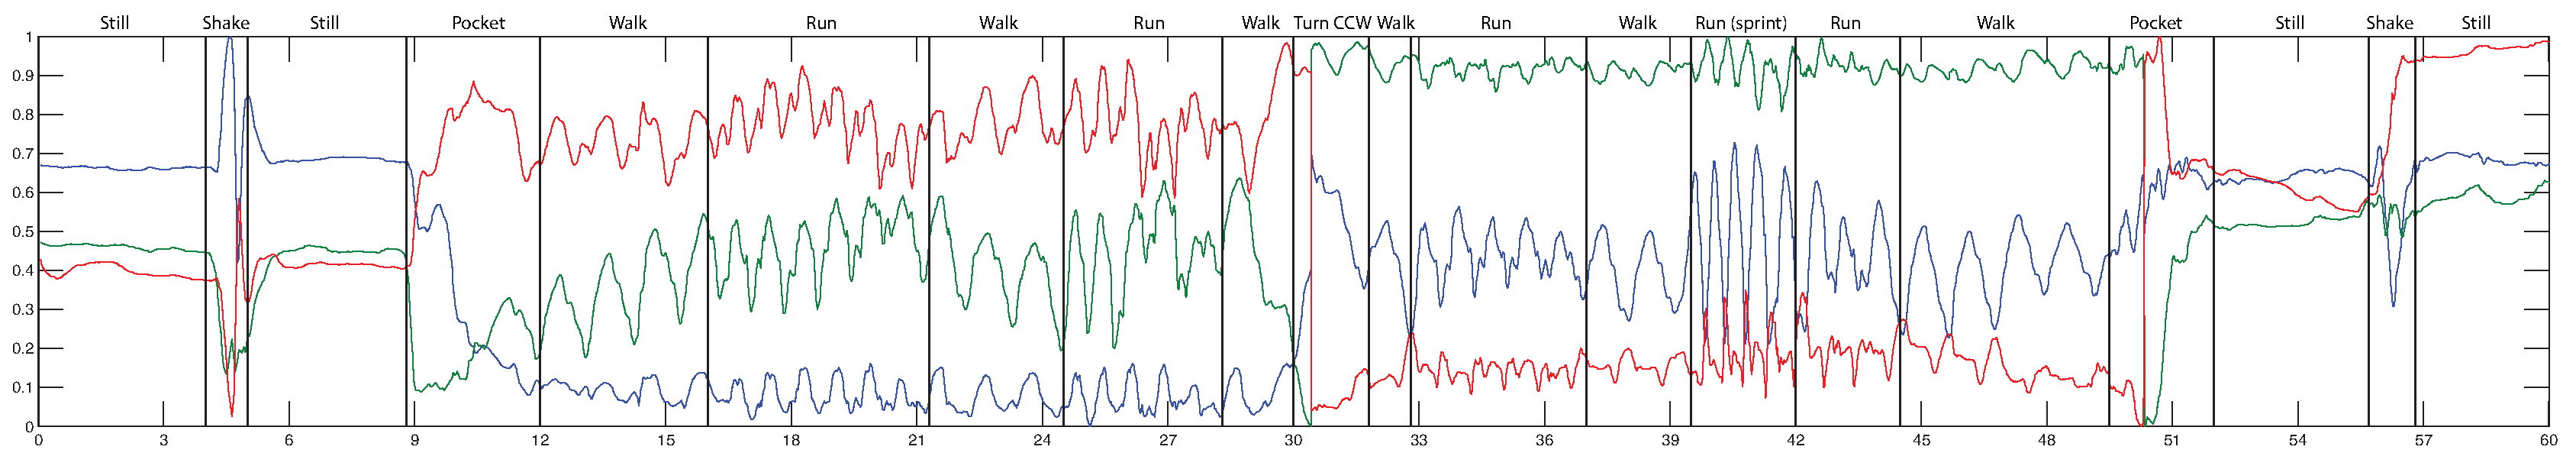
\includegraphics[width=1\textwidth]{./Figures/chapter6/data_collection/run-2-walk-run-jos/data_plot_rot_annotated.eps}
  \caption[R2: rotation]{Run 2: Walk-run-jos, rotation}
\end{figure}

\begin{figure}
\centering
  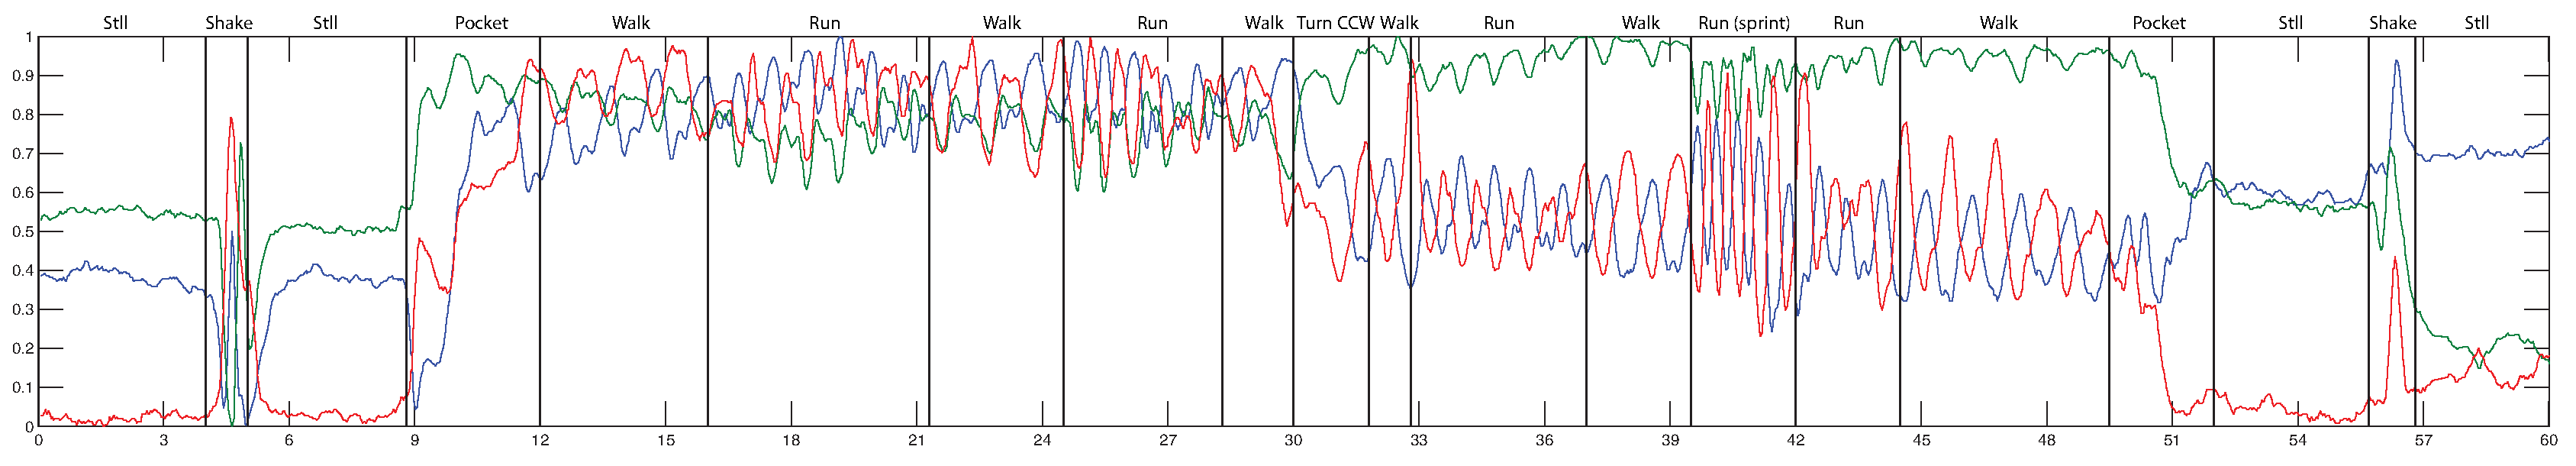
\includegraphics[width=1\textwidth]{./Figures/chapter6/data_collection/run-2-walk-run-jos/data_plot_mag_annotated.eps}
  \caption[R2: mag]{Run 2: Walk-run-jos, Mag}
\end{figure}

\begin{figure}
\centering
  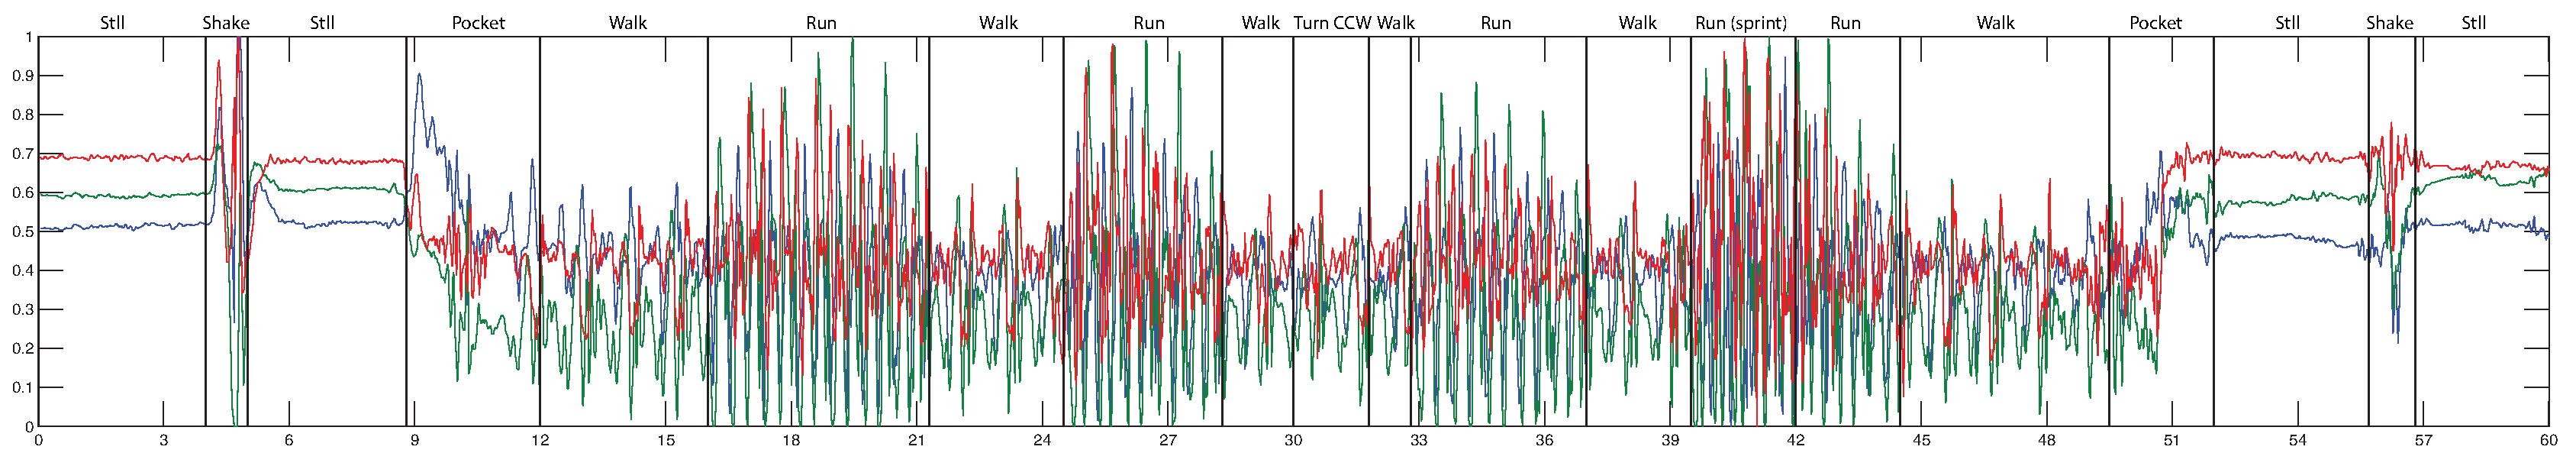
\includegraphics[width=1\textwidth]{./Figures/chapter6/data_collection/run-2-walk-run-jos/data_plot_acc_annotated.eps}
  \caption[R2: accelerometer]{Run 2: Walk-run-jos, accelerometer}
\end{figure}
% !TEX root = ../../main.tex
\section{Results}\label{sec:real_world_results}

\TODO{Add notion of \textbf{empirical} results.}

In the first paragraph we will explain that we use the same quality measures as used in \Cref{sec:artificial_data_quality_metrics} for objective tabular results.
We further argue that more important is the subjective, visual, inspection of the discovered change points regarding the sensor data.
To give both results, we will first give a table and box plot, like in \Cref{sec:artificial_data_results}.
After that, we will show characterizing parts of the plots with annotated and discovered change points.

\subsection{Objective measure}

\TODO{Table of search run (in the columns) and for each run the ratio of False Alarm Rate, Average benefit (closest CP) and STD benefit. Like chapter 5.}

\begin{table}
  \centering
  \begin{tabulary}{\textwidth}{|l|c|c|c|c|c|c|c|}
    \cline{2-8}
    \multicolumn{1}{l|}{} & Run 1 & Run 2 & Run 3 & Run 4 & Run 5 & Run 6 & Run 8 \\
    \hline
    Window length & 50 & 50 & 50 & 50 & 50 & 50 & 50 \\
    \hline
    Sigma of \gls{rbf} & 13 & 13 & 13 & 13 & 13 & 13 & 4 \\
    \hline
    High threshold & 1.2 & 1.5 & 1.3 & 1.1 & 1.3 & 1.2 & 1.7 \\
    \hline
    Low threshold & 0.8 & 0.8 & 0.6 & 0.7 & 0.7 & 0.8 & 0.6 \\
    \hline
    Closeness (s) & 0.7 & 0.85 & 1 & 0.6 & 0.7 & 1 & 0.8 \\
    \hline
    \hline
    $\operatorname*{far}(Y)$ & 0.1 & 0.05 & 0 & 0 & 0.2 & 0 & 0.48 \\
    \hline
    $\operatorname*{Average\_delay}$ & 0.52 & 0.83 & 0.47 & 0.92 & 1.26 & 1.05 & 0.92 \\
    \hline
    STD Delay & 0.29 & 0.55 & 0.52 & 0.75 & 1.67 & 0.78 & 0.92 \\
    \hline
  \end{tabulary}
  \caption[Results real world runs]{Parameter settings and results of the real-world data sets.}
  \label{tab:results_real_world}
\end{table}

Here something to refer to \Cref{fig:boxplot_real_world_runs}, about what it shows.

\begin{figure}
\centering
  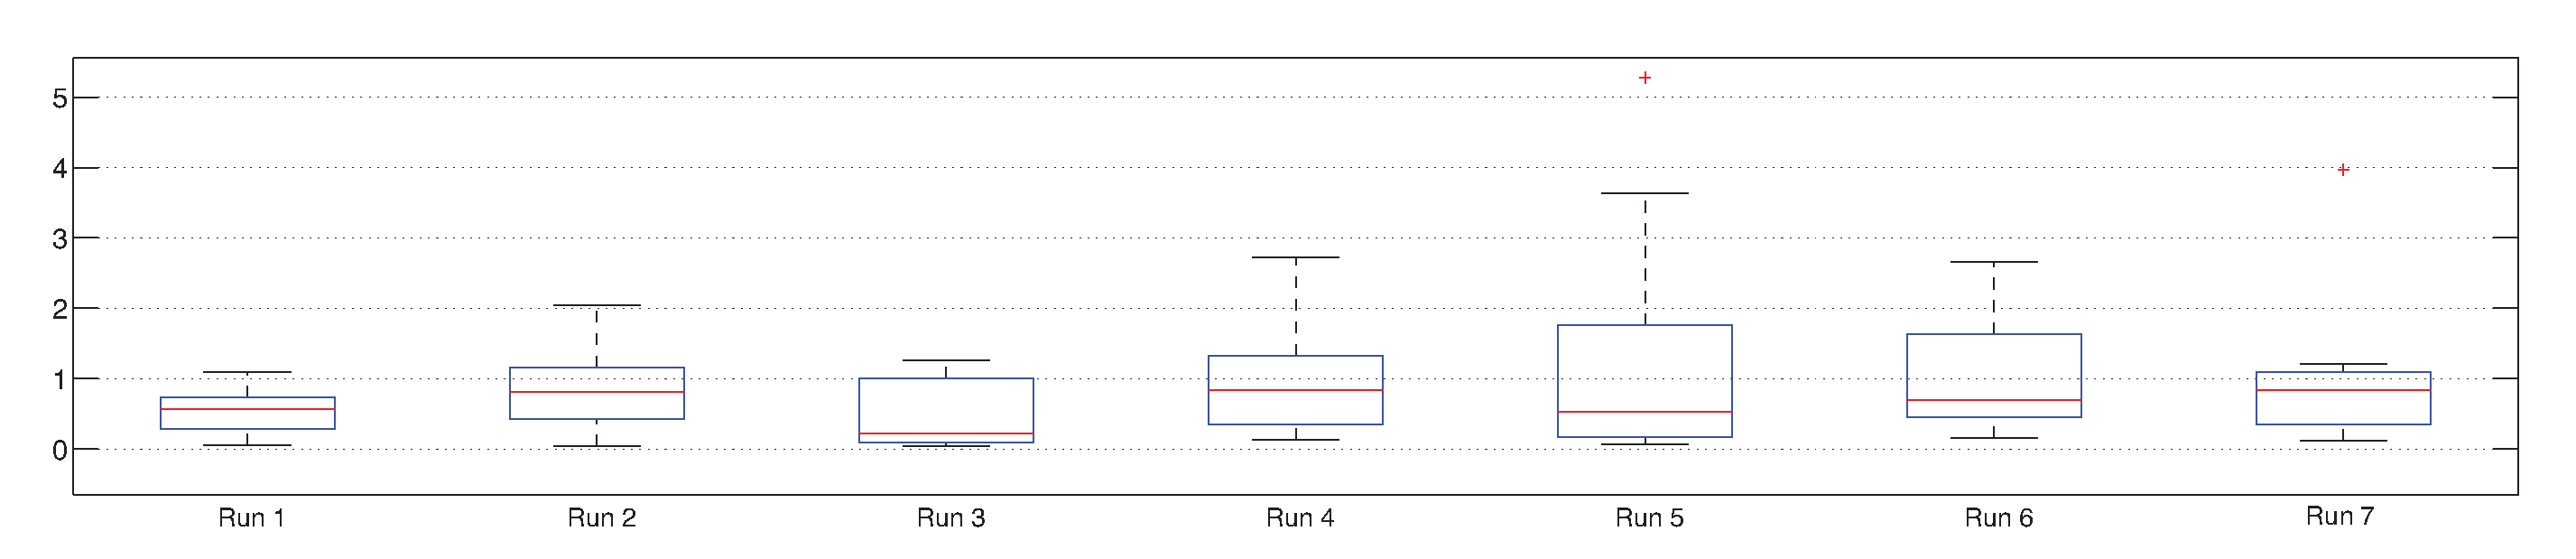
\includegraphics[width=1\textwidth]{./Figures/chapter6/data_collection/boxplot_results_real_world_runs.eps}
  \caption[Box plot results real-world runs]{Box plot of the results for the real-world runs, indicating the number of data points between the actual and closest detected change points. A lower and more compact box plot is better.}
  \label{fig:boxplot_real_world_runs}
\end{figure}

We will state observations and remarks from the results which present and applicable to all the runs.
After that, we will discuss special observations for each run individually.

\TODO{Uitleggen over sensitivity: we willen die zo laag mogelijk vanwege stabiliteit.}

About the overall performance and results, we have the following observations:
\begin{itemize}
  \item \textbf{Merging:} in our method we use a \emph{closeness} time period $t_c$ (usually up to $0.5$ - $1.0$ seconds) to merge discovered change points that have a very small distance between them.
  Multiple merging-strategies can be applied, and in our method we use the naive implementation by simply ignoring all the discovered change points that occur less than $t_c$ seconds after the previous change point.
  This works well when there is a block of noisy data with a high amount of (falsely) discovered change points.
  On the flip side, this method will ignore real new change points which occur during the noisy period.
  This problem on itself can be formulated as a change detection problem.
  \item \textbf{Masking:} Since the parameters for the detection method are set globally, it is difficult to discover all the change points (and only the change points) without a high \gls{far}.
  If a change point is proceeded by a noisy block, then the real change point will be merged with the previous change points.
  In an other case, where a change point is very clear represented in the data but the next, close by, other change point is more subtle, the latter change point is \emph{masked} by the former.
  This masking effect is also discussed in \cite{inclan1994use}, where an iterated approach is applied.
  \item \textbf{False heterogeneity:} For our video-data synchronization, we started and ended each recording with a few seconds in which the recording smartphone was kept still in the air.
  During this period, the data variance, and thus the constructed hypersphere, becomes very small.
  As a results, even small movements are considered to be changes and in the case of the mid-air still smartphone a lot of false change points are detected.
  Due to the merging effect described above, the final real change point (often shaking the smartphone) is not discovered.
  \item \textbf{Incorrect weighting:} In our analyses we have used the data from the accelerometer, magnetic field, and rotation sensors.
  In the segments which embodied movement in a circular manner (such as walking around a corner on the street, as in run 3 \TODO{add ref to image}), the turn was not discovered.
  Alternatively, when we only used the magnetic field and rotation sensors, the turn was correctly discovered.
  Other transitions, such as from walking to running, are harder to discover without the (linear) accelerometer sensor data.
\end{itemize}

\TODO{Add positive remarks}

When looking at the individual runs, we have the following observations for each run number:
\begin{enumerate}
  \item \textbf{Subject 2, straight}
    \begin{itemize}
      \item The first transition from running to walking, around $14s$ is harder to discover than the transition for the same activities around $33s$.
      This shows is that in real-world applications there is a diversity between the same transitions and activities.
      \item Around $8s$, $9s$, and $16s$ a few steps (while walking) are regarded as change points.
      During the running segments from $17s$ and $28s$ there is a lower probability of change for each step.
    \end{itemize}
  \item \textbf{Subject 1, straight}
    \begin{itemize}
      \item Following the video recordings, we have annotated a change point from running to walking around $37s$.
      Our method discovers a change point almost a second before.
      In retrospect, we can see that the data distribution indeed changes from the discovered change point on.
      This shows us two important principles.
      The first is that the annotations are very subjective.
      The second is that between different activities the transition period is longer than we would think.
      Looking at the data, we can see that the body slows down, even before we visually notice it on the video recordings.
    \end{itemize}
  \item \textbf{Subject 2, corner}
    \begin{itemize}
      \item The $90^{\circ}$ counter-clockwise turn during the walking activity is hard to discover when the accelerometer sensor data is included.
      When only the magnetic field and rotation sensors are used, the turn requires a lower sensitivity.
      With only these two sensors all the other change points in this run are also successfully discovered.
    \end{itemize}
  \item \textbf{Subject 2, fountain}
    \begin{itemize}
      \item Like in the first run, the walking segment from $24s$ results in a change point for each step.
      Further inspection of the data reveals that each step is indeed different from the other.
      Due to the global parameter settings, the sensitivity is too high for this segment to recognize it as one.
      \item During the circular run, from $12s$ till $24$, there are two change points discovered.
      The difference for the rotational vectors need to accumulate to a certain value before they have enough influence to let the rotation be regarded as a change point.
      \TODO{Beter formuleren}.
    \end{itemize}
  \item \textbf{Subject 1, fountain}
    \begin{itemize}
      \item As with the other runs, the accelerometer data makes it harder to detect turns.
      It requires a higher sensitivity, which results in a higher \gls{far}.
    \end{itemize}
  \item \textbf{Subject 2, fountain 2}
    \begin{itemize}
      \item During the standing segment around $38s$ there are a lot of false positives.
      It seems to be the \emph{false heterogeneity} problem described above.
    \end{itemize}
  \setcounter{enumi}{7}
  \item \textbf{Subject 3, indoor stairs}
    \begin{itemize}
      \item The walking segment around $22s$, between two segments of walking downstairs, shows little difference in the data.
      To recognize it as a change point a high sensitivity and low closeness time period $t_c$ is required.
      \item During some segments (downstairs from $24s$, upstairs from $42s$ and $54s$) the method discovers more change points than our annotation.
      A closer inspecting of the raw data reveals indeed changes in behavior.
      To exclude these (semi) false positives, a better tuning of parameters is required.
      \item Because of the circular shape of the stairs, the magnetic field sensors constantly differs.
      Although our method is build to exclude slow shifting changes (because we are only interested in sudden changes), with our used window width it still eventually results in change points.
      \item The difference between taking the stairs and walking is smaller than, \eg, walking and running.
      The delay between these segments seems to be larger, as illustrated around $33s$.
    \end{itemize}
\end{enumerate}

\TODO{Add suggestion for adaptive parameter tuning, locally determined}


Here comes a list of observations and conclusions on the performance:
\begin{itemize}
  \item \textbf{Perhaps something in bold:} here we list a funny observation.
  \eg that when walking the circulair stairs it is harder to find the rotation on the flat surface.
  \item Or just something else.
\end{itemize}

\subsection{Subjective measures}
In this subsection we will provide a few plots with characterizing parts of the sensor data, annotated change points, and discovered change points.
We use it to illustrate some aspects of the method, on which it performs well and where not.
We do not provide all plots, because that would take up to much time.
We do try to give a subjective conclusion about the performance, backed by the provided examples.


\subsection{Notes: remarks}
Mergen van change points:\\

Aanpak 1: Na ieder gevonden change point een bepaalde periode $s$ alle anderen negeren. Probleem: je hebt dan bijna altijd na $s$ sowieso een `gevonden' change point.\\
Aanpak 2: Alle change points die binnen $s$ van elkaar zitten mergen. Probleem: naar voren of naar achteren doen? Als je een heel lang blok hebt met CPs dicht bij elkaar, met mogelijk `echte' CPs, dan worden die ook genegeerd. Mogelijke oplossing: gebruik van `zekerheid' over de gevonden CPs om te mergen.

Het ghosting treedt vooral op aan het begin van iedere run, met het `kaliberen': het begin van de echte activiteit zit er te dicht op en wordt niet goed herkend.

Run 1 - Roemer\\

\begin{itemize}
  \item Doordat de thresholds niet adaptief zijn, wordt de gevoeligheid voor de hele methode globaal gezet.
  Dit zorgt dat ruwe overgangen gevonden worden, maar subtielere worden overgeslagen.
  Bijvoorbeeld: op 14s zit een overgang van rennen naar lopen, maar die is niet zo groot. Deze wordt niet gevonden, tenzij de gevoeligheid veel hoger gaat, maar dan krijg je weer teveel false positives. De overgang vlak erna, op 17s, gaat weer van lopen naar rennen en die wordt wel gevonden.
  \item Op 33s van rennen naar lopen wordt juist weer wel goed gevonden.
  \item Doordat in de data soms wel veranderingen zitten (die niet direct duidelijk zijn uit de video beelden) en change points dichtbij gemerged worden, kan er soms een groot verschil ontstaan. Bv op 8s en 9s. De changes op 7s en 10s worden gemist.
  \item De overgang van rennen naar sprint(?) op 31s wordt gemist.
\end{itemize}

Run 2 - Jos \\
\begin{itemize}
  \item Op 37s is een annotate van rennen naar lopen. De methode detecteert het bijna een seconde eerder. Als je naar de ruwe data kijkt zie je daar ook een verandering, dus nog voordat je het uit de video-beelden zou opmerken --> heel subjectief dus.
  \item Zelfde `ghosting' probleem als hierboven: bij overgang van Still naar Pocket wordt niets gevonden, doordat in de periode ervoor veel changes zijn. De data in `Still' is heel homogeen, dus kleine veranderingen worden als changes gezien, en die zijn er alsnog veel. --> \textbf{Hoe heterogener de data, hoe robuster}.
\end{itemize}

Run 3 - Roemer, around the corner \\
\begin{itemize}
  \item Met acc, mag, rot data is 90 graden CCW niet goed te vinden. Met mag,rot data wel --> te veel data is ook niet goed.
  \item Het enige punt, de draai, wordt met mag,rot goed gevonden. (geen plot of data, want verder niet interessant). Ook Walk-in-hand, pocket en Out-pocket worden erg nauwkeurig gevonden!
\end{itemize}

Run 4 - Roemer, fountain \\
\begin{itemize}
  \item Na 24s: van Rennen naar Lopen, worden meerdere change points gevonden. In de data zie je ook dat iedere stap een rustigere stap is, dus de gevoeligheid pakt dat op.
  \item De draaien in het Rennen rond 12s en 16s worden wel gevonden (bij hoge gevoeligheid, met delay), maar die rond 21s niet. (acc, mag, rot). Met alleen Rot ook niet.
  \item Correct number of change points found, but still 11 total difference. Would be better if benchmarking periods (still, shake) would not be present. (overall geldt dat ook).
  \item
\end{itemize}

Run 5 - Jos, fountain \\
\begin{itemize}
  \item Bij Acc,Mag,Rot worden de Turn CW punten niet goed gevonden. Bij alleen Rot wel (niet allemaal, maar wel beter).
  \item Om bij Acc,Mag,Rot de Turn te vinden is hoge gevoeligheid nodig, maar dat geeft hoge FAR.
  \item
\end{itemize}

Run 6 - Roemer, fountain \\
\begin{itemize}
  \item Om de overgang van rennen naar lopen op 18s te vinden is relatief hoge Low-threshold nodig (dus: hoge gevoeligheid).
  \item Bij hoge Low-Threshold wordt draai op 24s ook gevonden. Anders niet.
  \item Stilstaan op 38s geeft hele veel ruis in `thresholding' property. --> overgang naar lopen 2 sec later wordt niet goed gevonden. Komt doordat hypersphere heel klein wordt, en dus veel outliers?
  \item
\end{itemize}

Run 7 - Jos, fountain \\
Camera was leeg, dus mislukte run

Run 8 - Marc, indoor \\
\begin{itemize}
  \item Op 24s, van Walk naar Downstairs: door het ghosting effect is het moeilijk te pakken. Relatief hoge merging-tijd nodig, maar dat verwijderd deze, omdat het begin van lopen dicht zit op het begin van downstairs.
  \item Op 37s zit CCW Turn: is te herkennen (met acc, mag, rot) maar hoge gevoeligheid nodig.
  \item In tweede downstairs block (24s) en upstairs blocken (42s, 54s) worden halverwege ook changes gevonden (met acc, mag, rot). Ook met alleen Acc: zit ook echt verschil in de data
  \item Met alleen Mag data heel veel changes: cirkel-vorm van trap zorgt voor constante verandering.
  \item Overall: hoge FAR, door cirkelvorm trap (?)
  \item Verschil tussen down/upstairs en lopen is niet zo groot. Typisch: 33/34s: herkenning van overgang duurt even een stap.
  \item Vooral op einde, vanaf 66s (lopen naar stoel), heel veel False Positives. Veel verschillende activiteiten kort op elkaar.
\end{itemize}